\section{内部飛跡検出器}
%内部飛跡検出器は、加速器実験の衝突点を複数層に囲むようにして設置される粒子検出器の中で、最内層に設置される検出器である。
内部飛跡検出器は、検出器内に荷電粒子が通過すると、検出器内で電子正孔対が生成され、通過した情報として電気信号を出力することができる。
そのため、検出器に粒子が通過した情報を元に、粒子の飛跡を再構成することができる。
%粒子の飛跡からビームの衝突点、磁場による飛跡の曲率から粒子の運動量を測定することができる。
%測定から得られた情報から、衝突によって生成された粒子の性質や相互作用について調べることができる。

\begin{figure}[h]
    \centering
    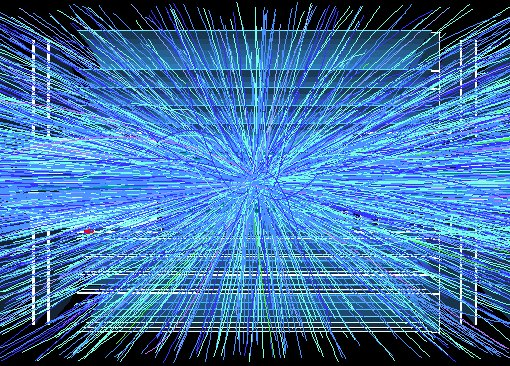
\includegraphics[width=10cm]{fig/ch1/HL-LHC_simulation.jpeg}
    \caption{HL-LHCの衝突点の様子\cite{HL-LHCsimulation}}
    \label{fg:HL-LHCsimulation}
\end{figure}

将来の加速器実験では、生成確率が低い粒子や質量が大きい粒子を発見するために、重心系エネルギーと衝突頻度を向上させる計画が検討されている。
加速器によって加速される粒子は、バンチと呼ばれる粒子の塊となっており、加速器実験ではその塊を衝突させている。
データ量の増加には、1バンチに含まれる粒子数を増やすことで衝突点の数を多くすることや、バンチとバンチの間隔を縮めて、衝突の頻度を高くすることが有効である。
現在のLHCでは1回のバンチ交差あたり最大60個の衝突が起きるが、
図\ref{fg:HL-LHCsimulation} のHL-LHCにおける衝突点のシミュレーション\cite{HL-LHCsimulation}では、
1バンチで200回の陽子-陽子衝突が生じるとシミュレーションされている。
HL-LHCに限った話ではなく、将来の加速器実験を見据えた際には、さらなる衝突回数の増加があると考えられる。
粒子の衝突によって生じる事象のほとんどが背景事象で、その中から調べたい衝突を見つけなければならない。
内部飛跡検出器には大量の粒子が通過するため、その情報から粒子1つ1つの飛跡を再構成できるような性能が求められる。
加速器の高輝度化に対応できる内部飛跡検出器の開発が必要不可欠である。

HL-LHC実験で使われるATLAS検出器では、主に電極サイズが$50 \mu\rm{m}$×$50 \mu\rm{m}$のピクセル検出器を使用する。
検出器の電極サイズを細かくすることで、位置分解能を向上とoccupancyを下げることができるため、
多数の衝突から生成される粒子の飛跡をより確実に再構成できる。
高い位置分解能に加えて、検出器に高い時間分解能を持たせることで粒子の飛跡に時間情報を追加することができる。
図\ref{fg:4DTracking} に位置情報と時間情報を用いて飛跡を再構成した様子を示す。
\begin{figure}[h]
    \centering
    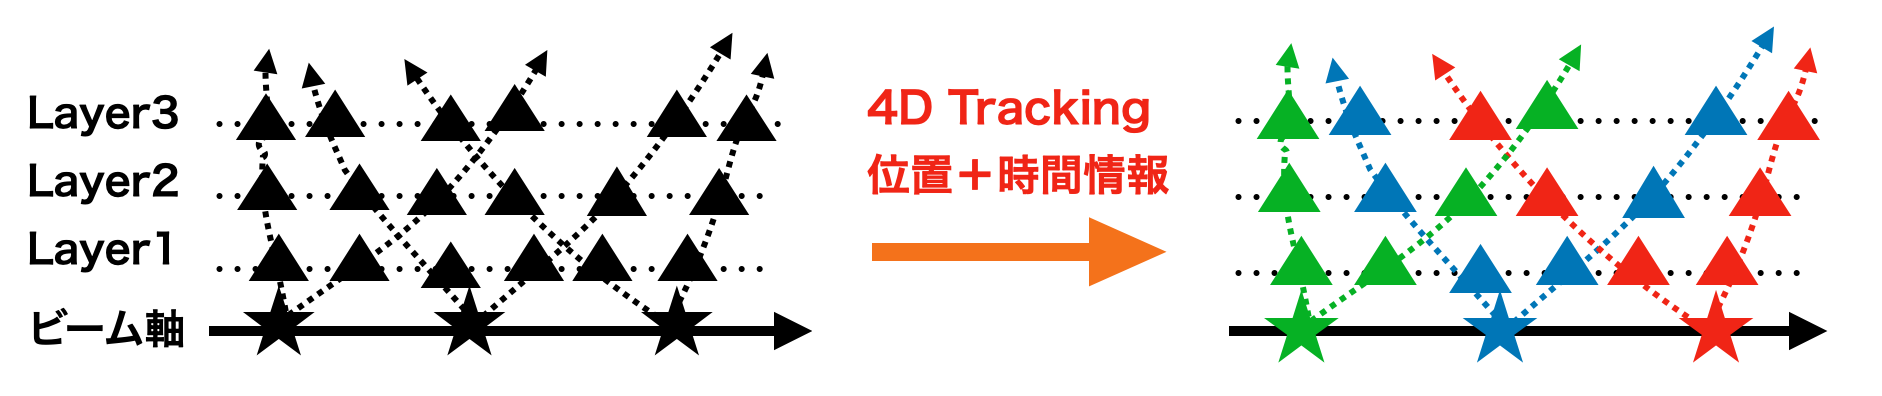
\includegraphics[width=16cm]{fig/ch1/4DTracking_new.png}
    \caption[位置情報と時間情報による飛跡の再構成の様子]{位置情報と時間情報による飛跡の再構成の様子。星印が粒子のヒット情報で点線が再構成した飛跡である。\\時間分解能を持たせた検出器を用いることで、飛跡と衝突点を時間で区別することができる様子を示している。}
    \label{fg:4DTracking}
\end{figure}
星印が衝突点で、三角が粒子のヒット情報である。
検出器が3層に設置されており、ビーム軸上で起きた衝突から3つの検出器がヒット情報を得ることで、飛跡を再構成した様子点線が再構成した飛跡である。
左の図が時間情報のない場合で、右の図が時間情報がある場合の様子である。
時間情報があることで、飛跡の再構成することに加えて、右の図で衝突点と飛跡を色で区別したように、時間で区別することが可能になる。

図\ref{fg:4Dtrack_ATLAS} には、HL-LHCのATLAS実験による衝突点のシミュレーション結果を示す\cite{ATL-PHYS-PUB-2023-023}。
左の図が位置分解能による飛跡の再構成で、右の図が位置分解能と時間分解能による飛跡の再構成を示している。
時間分解能が加わることによって、衝突点と飛跡の時間情報の取得により、粒子密度が高い状況でも高輝度化に伴うパイルアップによって困難とされる、飛跡の再構成が可能となる。
1 cm単位で検出器を設置する場合、光速で進む粒子の飛跡に時間情報を加えるためには、30 psの時間分解能を満たす必要がある。
加速器の高輝度化に対して、高い時間分解能と位置分解能を併せ持つ内部飛跡検出器が非常に有効であり、新粒子や新物理の発見に大きく貢献することができる。

\begin{figure}[h]
    \begin{minipage}[b]{0.5\linewidth}
        \centering
        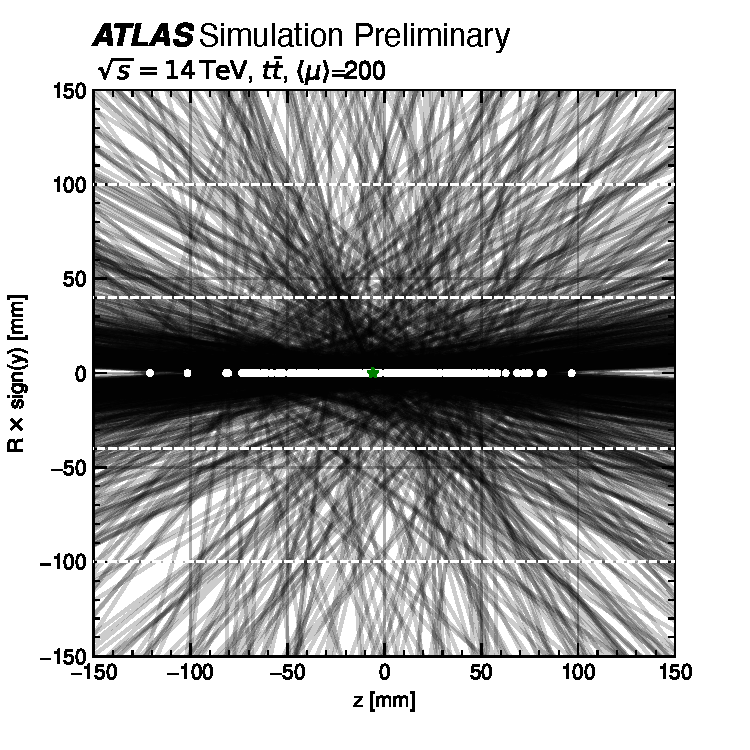
\includegraphics[scale=0.5]{fig/ch1/ATLAS_3Dtrack.pdf}
        \subcaption{位置分解能による飛跡の再構成}
        \label{fg:ATLAS_3Dtrack}
    \end{minipage}
    \begin{minipage}[b]{0.5\linewidth}
        \centering
        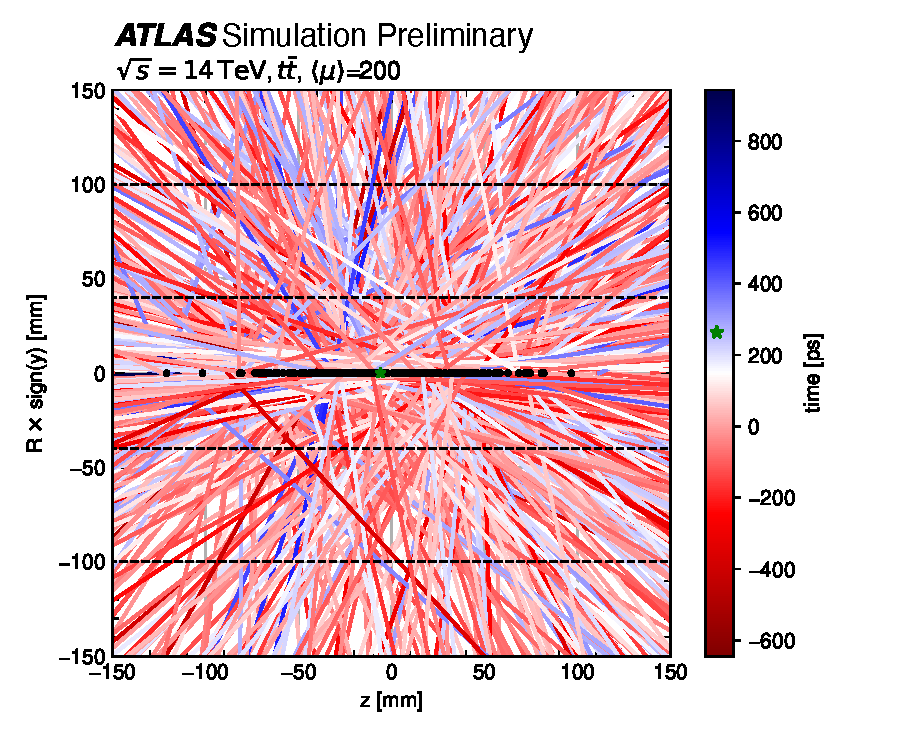
\includegraphics[scale=0.5]{fig/ch1/ATLAS_4Dtrack.pdf}
        \subcaption{位置分解能と時間分解能による飛跡の再構成}
        \label{fg:ATLAS_4Dtrack}
    \end{minipage}
    \caption[飛跡の再構成のシミュレーション\cite{ATL-PHYS-PUB-2023-023}]{飛跡の再構成のシミュレーション\cite{ATL-PHYS-PUB-2023-023}\\時間分解能があることで、衝突点と飛跡がどのタイミングで起こったのかがわかる。粒子密度が高くなっても衝突点と飛跡の紐付けが可能。}
    \label{fg:4Dtrack_ATLAS}
\end{figure}


